\chapter{Operadores, observables y matrices de Pauli}

La buena notación no es un adorno. En una disciplina basada en vectores abstractos y números complejos, una notación que nos permite manipular símbolos sin tener que traducirlos continuamente a palabras forma parte del propio instrumental. La notación de bra--ket de Dirac es valiosa precisamente por esta razón: mantiene visible la geometría del espacio de estados y, a la vez, nos permite calcular con componentes y matrices.

Nuestra tarea inmediata es matemática. Introduciremos los operadores lineales, aprenderemos cómo actúan tanto sobre los bras como sobre los kets y aislaremos la clase especial llamada operadores hermíticos. Solo entonces asignaremos significado físico a las palabras \emph{observable}, \emph{resultado de una medición} y \emph{probabilidad}. Así, las tres observables de espín aparecerán como matrices de Pauli, en lugar de presentarse como objetos que debamos memorizar.

\section{Bases ortonormales y componentes}

Los estados forman un espacio vectorial complejo. Sus vectores ket se pueden sumar y multiplicar por números complejos. A cada ket \(\ket{A}\) le corresponde un bra \(\bra{A}\), obtenido mediante la operación de conjugación dual. La base no es única, pero, una vez elegida, todo vector puede describirse mediante sus componentes en ella.

Sea
\[
\bigl\{\ket{1},\ket{2},\ldots,\ket{N}\bigr\}
\]
una base ortonormal. La ortogonalidad y la normalización se resumen en
\begin{equation}
\braket{j}{i}=\delta_{ji}.
\label{eq:orthonormal-basis}
\end{equation}
Aquí, \(\delta_{ji}\) vale uno cuando \(j=i\) y cero en caso contrario. La dimensión \(N\) es el número máximo de direcciones mutuamente ortogonales del espacio; una base ortonormal completa contiene exactamente ese número de vectores.

Desarrollemos un ket arbitrario:
\begin{equation}
\ket{A}=\sum_i \alpha_i\ket{i}.
\label{eq:ket-expansion}
\end{equation}
Los coeficientes no tienen nada de misterioso. Multipliquemos por la izquierda por \(\bra{j}\):
\begin{align}
\braket{j}{A}
 &=\sum_i\alpha_i\braket{j}{i} \\
 &=\sum_i\alpha_i\delta_{ji}
 =\alpha_j.
\end{align}
Por tanto,
\begin{equation}
\alpha_i=\braket{i}{A}.
\label{eq:components-inner-products}
\end{equation}
La componente \(i\)-ésima es la proyección de \(\ket{A}\) sobre la dirección \(i\)-ésima de la base.

Al sustituir la Ecuación~\eqref{eq:components-inner-products} en la Ecuación~\eqref{eq:ket-expansion} obtenemos una forma especialmente útil:
\begin{equation}
\ket{A}=\sum_i\ket{i}\braket{i}{A}.
\label{eq:ket-completeness-action}
\end{equation}
La suma no ha modificado el vector; solo lo ha descompuesto en las direcciones de la base para luego reconstruirlo. Repetiremos esta operación muchas veces. Suele describirse como \emph{insertar un conjunto completo de estados}, porque
\begin{equation}
\sum_i\ket{i}\bra{i}=\mathbf 1.
\label{eq:resolution-identity}
\end{equation}

El desarrollo correspondiente para el bra es
\begin{equation}
\bra{A}=\sum_i\braket{A}{i}\bra{i}
       =\sum_i\alpha_i^*\bra{i}.
\label{eq:bra-expansion}
\end{equation}
La conjugación compleja de \(\alpha_i\) es esencial. Al convertir un ket en bra se conjuga cada coeficiente numérico.

\begin{figure}[htbp]
\centering
\includegraphics[width=0.82\textwidth]{lecture_03_figure_04.png}
\caption{Las dos reglas que definen un operador lineal, escritas después del repaso de las bases.}
\lectureframe{00:12:44}
\end{figure}

\section{Operadores lineales como máquinas}

Un operador lineal \(M\) es una regla que asigna un ket de salida único a cada ket de entrada. Una imagen útil, propuesta por John Wheeler, es la de una máquina con un puerto de entrada y otro de salida: introducimos \(\ket{A}\), hacemos girar la máquina y obtenemos \(M\ket{A}\). La entrada determina la salida. La operación inversa no tiene por qué ser única: dos entradas pueden producir la misma salida, y puede que no exista una máquina inversa.

El adjetivo \emph{lineal} se refiere a dos reglas. Para un número complejo \(z\),
\begin{align}
M\bigl(z\ket{A}\bigr)&=z\,M\ket{A}, \label{eq:operator-homogeneous}\\
M\bigl(\ket{A}+\ket{B}\bigr)&=M\ket{A}+M\ket{B}.
\label{eq:operator-additive}
\end{align}
El escalar atraviesa la máquina sin cambios, y la suma se puede procesar término a término. Estas reglas implican también la linealidad para cualquier combinación lineal compleja finita.

La misma idea se aplica a los vectores ordinarios tridimensionales. La mecánica cuántica no inventa las aplicaciones lineales. Las vuelve indispensables porque el espacio de estados es abstracto y complejo, y porque las magnitudes medibles se representarán mediante una familia destacada de tales aplicaciones.

\section{De un operador a su matriz}

Supongamos que la máquina transforma \(\ket{A}\) en \(\ket{B}\):
\begin{equation}
M\ket{A}=\ket{B}.
\label{eq:operator-action}
\end{equation}
Elijamos la misma base ortonormal para la entrada y la salida, y escribamos
\[
\ket{A}=\sum_j\alpha_j\ket{j},
\qquad
\ket{B}=\sum_i\beta_i\ket{i}.
\]
Para hallar la componente de salida \(i\)-ésima, proyectemos la Ecuación~\eqref{eq:operator-action} con \(\bra{i}\):
\begin{equation}
\bra{i}M\ket{A}=\braket{i}{B}=\beta_i.
\end{equation}
Ahora insertemos el desarrollo de \(\ket{A}\):
\begin{align}
\bra{i}M\ket{A}
 &=\sum_j\bra{i}M\ket{j}\braket{j}{A}\\
 &=\sum_j\bra{i}M\ket{j}\alpha_j
 =\beta_i.
\end{align}
Los números
\begin{equation}
m_{ij}\equiv\bra{i}M\ket{j}
\label{eq:matrix-elements}
\end{equation}
son los \emph{elementos de matriz} de \(M\) en la base elegida. En consecuencia,
\begin{equation}
\boxed{\sum_jm_{ij}\alpha_j=\beta_i.}
\label{eq:component-action}
\end{equation}

\begin{figure}[htbp]
\centering
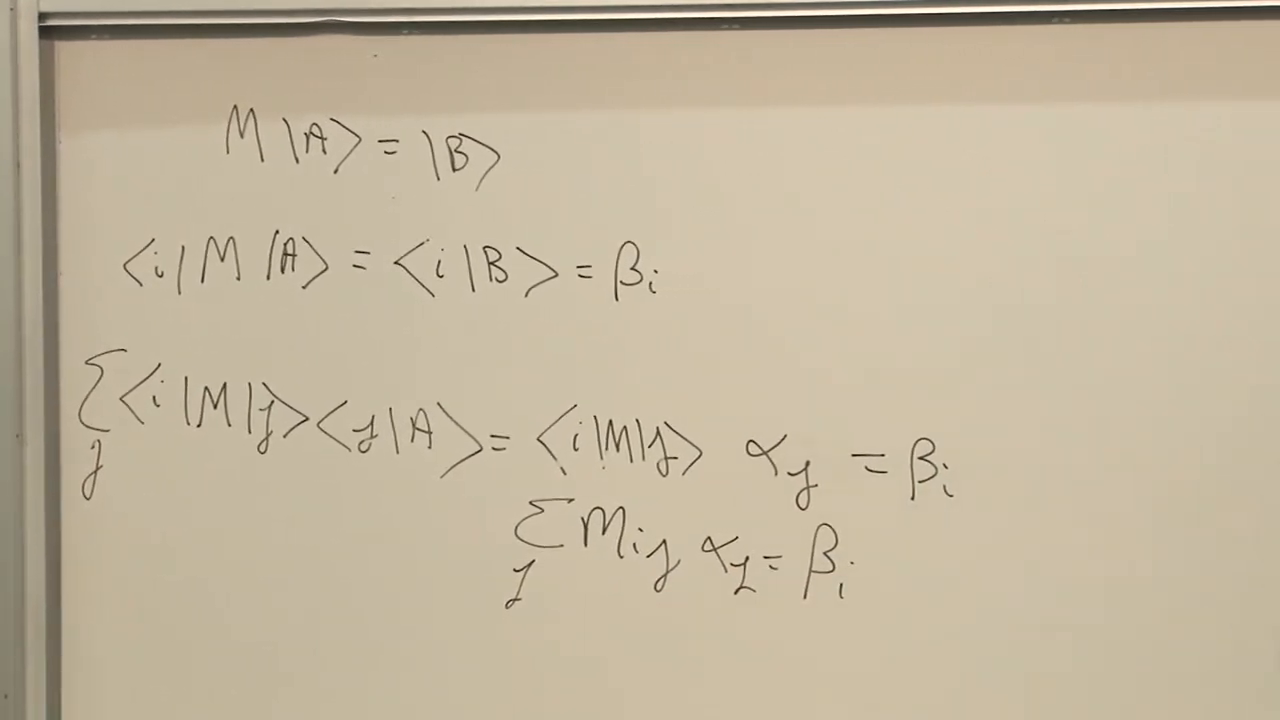
\includegraphics[width=0.84\textwidth]{lecture_03_figure_02.png}
\caption{La ecuación abstracta \(M\ket{A}=\ket{B}\), proyectada y descompuesta en la regla para las componentes \(\sum_jm_{ij}\alpha_j=\beta_i\).}
\lectureframe{00:18:30}
\end{figure}

Si el espacio tiene dimensión \(N\), los \(N^2\) números \(m_{ij}\) forman una matriz cuadrada \(N\times N\). La Ecuación~\eqref{eq:component-action} es precisamente
\begin{equation}
\begin{pmatrix}
m_{11}&m_{12}&\cdots&m_{1N}\\
m_{21}&m_{22}&\cdots&m_{2N}\\
\vdots&\vdots&\ddots&\vdots\\
m_{N1}&m_{N2}&\cdots&m_{NN}
\end{pmatrix}
\begin{pmatrix}
\alpha_1\\
\alpha_2\\
\vdots\\
\alpha_N
\end{pmatrix}
=
\begin{pmatrix}
\beta_1\\
\beta_2\\
\vdots\\
\beta_N
\end{pmatrix}.
\label{eq:matrix-vector-action}
\end{equation}
Para obtener \(\beta_1\), multipliquemos la primera fila por la columna de entrada y sumemos sus términos; repitamos el procedimiento con la segunda fila para obtener \(\beta_2\), y así sucesivamente. La matriz es la versión concreta de la máquina de Wheeler.

\begin{figure}[htbp]
\centering
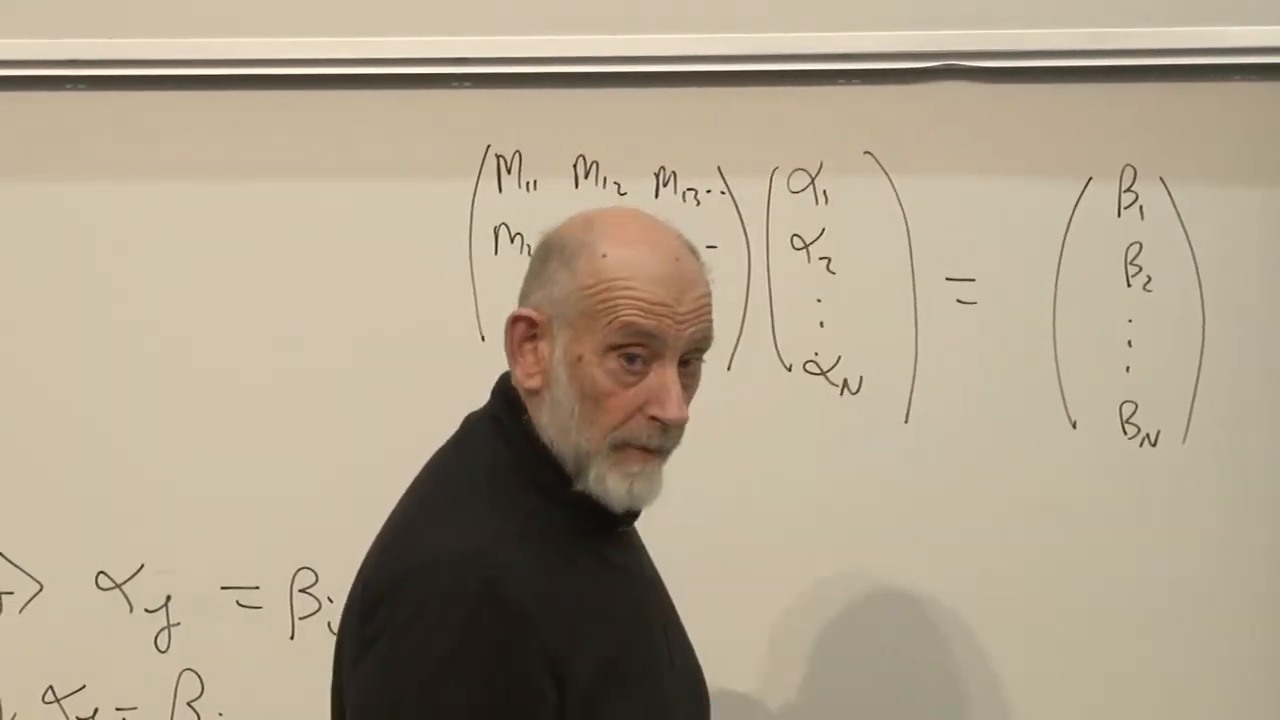
\includegraphics[width=0.84\textwidth]{lecture_03_figure_03.png}
\caption{La misma acción del operador representada como una matriz cuadrada que multiplica la columna de coeficientes de entrada.}
\lectureframe{00:20:01}
\end{figure}

Hemos ganado un algoritmo, pero la geometría ya no resulta tan visible. La afirmación abstracta \(M\ket{A}=\ket{B}\) no depende de las coordenadas. Las entradas concretas \(m_{ij}\), \(\alpha_j\) y \(\beta_i\) sí dependen de la base elegida. Una base ortonormal distinta cambia los tres conjuntos de componentes, pero deja inalterados la aplicación subyacente y sus predicciones físicas.

\begin{classroomqa}
\audiencequestion{¿Puede la elección de la base determinar si un problema se puede resolver?}
\lecturerresponse{Puede determinar si la solución se ve con facilidad. Una base bien elegida puede diagonalizar un operador y hacer que el cálculo sea casi inmediato; una base inadecuada puede ocultar la estructura bajo un álgebra engorrosa. Pero no puede cambiar el resultado de un experimento. Si dos bases conducen a respuestas físicas distintas, el cálculo es incorrecto.}
\end{classroomqa}

\section{Bras, kets y antilinealidad}

\begin{classroomqa}
\audiencequestion{¿Puede un operador lineal transformar un ket en un bra, o un bra en un ket?}
\lecturerresponse{No, si se trata de un operador lineal ordinario de los que acabamos de definir. Este transforma kets en kets y deja pasar los escalares complejos sin modificarlos. La operación que intercambia kets y bras también conjuga sus coeficientes, por lo que pertenece a otra clase.}
\end{classroomqa}

La multiplicación por un número complejo fijo es un operador lineal sencillo. La conjugación compleja no lo es. Si \(K\) denota la conjugación, entonces
\[
K\bigl(z\ket{A}\bigr)=z^*K\ket{A},
\]
pero no \(zK\ket{A}\). Esta aplicación se llama \emph{antilineal}. El nombre no significa que sea lo contrario de lineal; indica que conjuga los escalares. Su relación más profunda con las antipartículas queda fuera del tema de esta exposición.

Sin embargo, podemos definir la acción de operadores lineales sobre bras. Por convención, el operador se escribe a la derecha:
\begin{equation}
\bra{A}M.
\end{equation}
La definición se elige de modo que los elementos de matriz no presenten ambigüedades de agrupación:
\begin{equation}
\bra{A}\bigl(M\ket{B}\bigr)
=
\bigl(\bra{A}M\bigr)\ket{B}
\equiv
\bra{A}M\ket{B}.
\label{eq:bracket-independence}
\end{equation}

Veamos por qué esto es posible: desarrollemos ambos vectores:
\begin{align}
\bra{A}M\ket{B}
 &=\left(\sum_i\alpha_i^*\bra{i}\right)
   M
   \left(\sum_j\beta_j\ket{j}\right)\\
 &=\sum_{ij}\alpha_i^*m_{ij}\beta_j.
\label{eq:matrix-element-double-sum}
\end{align}
Se trata de una suma doble ordinaria. Podemos sumar primero respecto de \(j\) e interpretar que \(M\) actúa sobre el ket, o sumar primero respecto de \(i\) e interpretar que actúa sobre el bra. El resultado es el mismo. La notación se dispuso precisamente así para poder eliminar los paréntesis innecesarios.

\section{La operación daga}

Hay otra cuestión, distinta, sobre la acción en el lado del bra. Supongamos que
\[
M\ket{A}=\ket{B}.
\]
¿Qué operador transforma el bra correspondiente \(\bra{A}\) en \(\bra{B}\)? En general, no es \(M\) mismo. Si \(M\) fuera la multiplicación por un número complejo \(z\), la ecuación para el ket sería \(\ket{B}=z\ket{A}\), mientras que la ecuación para el bra sería \(\bra{B}=z^*\bra{A}\).

El operador requerido se denota \(M^\dagger\) y se llama \emph{conjugado hermítico} de \(M\). Se define mediante
\begin{equation}
M\ket{A}=\ket{B}
\quad\Longleftrightarrow\quad
\bra{A}M^\dagger=\bra{B}.
\label{eq:dagger-definition}
\end{equation}
La daga es el análogo, para operadores, de la conjugación compleja.

La regla para las matrices se obtiene directamente. Sea
\[
M\ket{i}=\ket{i'}.
\]
Entonces,
\[
m_{ji}=\bra{j}M\ket{i}=\braket{j}{i'}.
\]
La relación para el bra conjugado mediante la daga es \(\bra{i}M^\dagger=\bra{i'}\), así que
\[
(m^\dagger)_{ij}
=\bra{i}M^\dagger\ket{j}
=\braket{i'}{j}.
\]
Al invertir el orden de un producto interno, se obtiene su conjugado complejo:
\[
\braket{i'}{j}=\braket{j}{i'}^*.
\]
Por tanto,
\begin{equation}
\boxed{(m^\dagger)_{ij}=m_{ji}^*.}
\label{eq:dagger-matrix-elements}
\end{equation}

\begin{figure}[htbp]
\centering
\includegraphics[width=0.84\textwidth]{lecture_03_figure_05.png}
\caption{La relación completa para el conjugado hermítico: intercambiar los índices y tomar el conjugado complejo.}
\lectureframe{00:42:23}
\end{figure}

En el lenguaje de matrices, primero trasponemos y luego tomamos el conjugado complejo:
\begin{equation}
\begin{pmatrix}
a&b\\
c&d
\end{pmatrix}^{\!\dagger}
=
\begin{pmatrix}
a^*&c^*\\
b^*&d^*
\end{pmatrix}.
\label{eq:dagger-two-by-two}
\end{equation}
La trasposición refleja las entradas respecto de la diagonal principal; la conjugación reemplaza cada \(i\) por \(-i\). Por ejemplo,
\begin{equation}
\begin{pmatrix}
2&6+7i\\
4-i&9+i
\end{pmatrix}^{\!\dagger}
=
\begin{pmatrix}
2&4+i\\
6-7i&9-i
\end{pmatrix}.
\label{eq:dagger-numerical-example}
\end{equation}
Las entradas diagonales conservan su posición, pero se conjugan; las dos entradas fuera de la diagonal intercambian posiciones y también se conjugan.

\section{Operadores hermíticos}

Un número complejo es real si y solo si es igual a su propio conjugado complejo. El análogo para operadores es inmediato.

\begin{definition}
Un operador \(M\) es \emph{hermítico} cuando
\begin{equation}
M=M^\dagger.
\label{eq:hermitian-definition}
\end{equation}
De forma equivalente, en toda base ortonormal,
\begin{equation}
m_{ij}=m_{ji}^*.
\label{eq:hermitian-components}
\end{equation}
\end{definition}

Tomemos \(i=j\) en la Ecuación~\eqref{eq:hermitian-components}. Entonces,
\[
m_{ii}=m_{ii}^*,
\]
por lo que todas las entradas diagonales son reales. Fuera de la diagonal, las entradas aparecen en pares reflejados conjugados. Si una entrada es \(4-i\), su pareja reflejada es \(4+i\); si una es el número real \(5\), también lo es su pareja.

\begin{figure}[htbp]
\centering
\includegraphics[width=0.78\textwidth]{lecture_03_figure_06.png}
\caption{Un ejemplo completo de matriz hermítica: entradas reales en la diagonal y pares de entradas complejas conjugadas reflejadas respecto de ella.}
\lectureframe{00:45:43}
\end{figure}

Los operadores hermíticos son importantes porque representarán magnitudes medibles. Antes de establecer esa correspondencia, necesitamos entender sus direcciones propias.

\section{Vectores propios y direcciones propias}

La primera vez que uno se encuentra con los vectores propios, esta parte puede parecer más rápida que la física que la rodea. Las ideas pertenecen al álgebra lineal estándar, no constituyen una nueva hipótesis física; si no le resultan familiares, conviene repasar con calma las definiciones y luego volver al argumento.

Un operador general cambia la dirección de un vector. Por ejemplo, una rotación en el espacio tridimensional ordinario hace que casi cualquier vector cambie de dirección. El eje de rotación es una excepción: un vector paralelo a ese eje conserva su dirección. Este es el modelo de un vector propio.

Una rotación no trivial de un plano real bidimensional ilustra la posibilidad opuesta: no hay ninguna dirección real que permanezca fija salvo por un factor de escala real. Así, un operador genérico en un espacio real restringido no tiene por qué tener un vector propio real. Los operadores hermíticos en los espacios complejos de estados que se usan en mecánica cuántica tienen propiedades mucho más fuertes.

Un vector propio de \(M\) satisface
\begin{equation}
M\ket{i}=\lambda_i\ket{i}.
\label{eq:eigenvalue-equation}
\end{equation}
El número \(\lambda_i\) es su valor propio. El vector propio pertenece al operador; no se habla de un vector propio sin especificar la aplicación cuya dirección conserva.

La Ecuación~\eqref{eq:eigenvalue-equation} no fija ni su longitud ni su fase. Para todo número complejo no nulo \(z\),
\[
M\bigl(z\ket{i}\bigr)
=zM\ket{i}
=\lambda_i\bigl(z\ket{i}\bigr).
\]
Por eso es más preciso hablar de una \emph{dirección propia}: todo múltiplo no nulo de \(\ket{i}\) describe la misma dirección y tiene el mismo valor propio. Normalmente elegimos un representante normalizado.

El hecho espectral fundamental es el siguiente: un operador hermítico en un espacio vectorial complejo de dimensión \(N\) tiene una base ortonormal completa formada por \(N\) vectores propios. Podemos ver dos partes de esta afirmación con muy poco álgebra.

\subsection{Los valores propios de un operador hermítico son reales}

Supongamos que \(M=M^\dagger\) y que
\[
M\ket{i}=\lambda_i\ket{i}.
\]
Tomemos el conjugado hermítico de toda la ecuación:
\begin{equation}
\bra{i}M^\dagger=\lambda_i^*\bra{i}.
\label{eq:eigen-bra-equation}
\end{equation}
Como \(M^\dagger=M\), multipliquemos la ecuación para el ket por \(\bra{i}\) y la ecuación para el bra por \(\ket{i}\):
\begin{align}
\bra{i}M\ket{i}&=\lambda_i\braket{i}{i},\\
\bra{i}M\ket{i}&=\lambda_i^*\braket{i}{i}.
\end{align}
El mismo factor, la norma no nula, multiplica ambos números; por tanto,
\begin{equation}
\lambda_i=\lambda_i^*.
\end{equation}
Todo valor propio de un operador hermítico es real. Esta es la primera señal de que un operador así puede representar el número real que muestra un aparato de medida.

\subsection{Los valores propios distintos corresponden a vectores propios ortogonales}

Sean
\[
M\ket{i}=\lambda_i\ket{i},
\qquad
M\ket{j}=\lambda_j\ket{j},
\]
donde \(M\) es hermítico. Tomemos el conjugado hermítico de la segunda ecuación. Ya sabemos que su valor propio es real:
\[
\bra{j}M=\lambda_j\bra{j}.
\]
Ahora multipliquemos la primera ecuación por \(\bra{j}\) y la ecuación para el bra por \(\ket{i}\):
\begin{align}
\bra{j}M\ket{i}&=\lambda_i\braket{j}{i},\\
\bra{j}M\ket{i}&=\lambda_j\braket{j}{i}.
\end{align}
Al restar, obtenemos
\begin{equation}
\boxed{(\lambda_i-\lambda_j)\braket{j}{i}=0.}
\label{eq:hermitian-orthogonality}
\end{equation}
Si \(\lambda_i\ne\lambda_j\), entonces
\[
\braket{j}{i}=0.
\]
Las direcciones propias son ortogonales.

\begin{figure}[htbp]
\centering
\includegraphics[width=0.82\textwidth]{lecture_03_figure_07.png}
\caption{La línea decisiva de la demostración de ortogonalidad: los valores propios distintos obligan a que el producto interno se anule.}
\lectureframe{00:59:00}
\end{figure}

Cuando dos valores propios coinciden, la Ecuación~\eqref{eq:hermitian-orthogonality} no impone ninguna condición dentro de ese subespacio propio degenerado. Allí se puede elegir una base ortonormal. Junto con las demás direcciones propias, esos vectores forman la base ortonormal completa de vectores propios que garantiza el teorema espectral.

La ortogonalidad también tiene una interpretación física. Dos estados ortogonales se pueden distinguir sin ambigüedad mediante una medición adecuada. Los estados propios con valores propios distintos tienen que ser distinguibles, porque el aparato indica para cada uno un número real diferente. El álgebra y el significado operacional ya apuntan a la misma correspondencia.

\section{Los postulados de la medición}

Ya tenemos el formalismo suficiente para enunciar las correspondencias fundamentales de la mecánica cuántica. Al principio pueden sonar ajenas. Su significado solo se concreta cuando las aplicamos; enunciémoslas con claridad y volvamos enseguida al experimento de espín.

Una medición produce un número real. Se pueden reunir dos lecturas reales compatibles en un número complejo, pero ese número sigue representando dos mediciones. El resultado elemental de un detector es real. Por eso los operadores hermíticos son candidatos naturales: sus valores propios son reales y sus vectores propios forman una base ortonormal completa.

\begin{enumerate}\item Una magnitud medible, u \emph{observable}, se representa mediante un operador hermítico \(M\).
\item Los posibles resultados de medir \(M\) son sus valores propios \(\lambda_i\).
\item Un estado en el que \(M\) tiene el valor definido \(\lambda_i\) es un estado propio \(\ket{i}\) que satisface
\[
M\ket{i}=\lambda_i\ket{i}.
\]
\item Si el sistema se encuentra en un estado general normalizado \(\ket{A}\), la probabilidad de obtener \(\lambda_i\) es
\begin{equation}
P(\lambda_i\mid A)
=\left|\braket{i}{A}\right|^2
=\braket{i}{A}\braket{A}{i}.
\label{eq:born-rule}
\end{equation}\end{enumerate}

Esta lista es un punto de partida práctico, no necesariamente un sistema mínimo de axiomas independientes; con una formulación más económica, algunas afirmaciones se pueden deducir de otras. Mantener separadas las correspondencias facilita ver sus funciones físicas.

El número complejo \(\braket{i}{A}\) es una \emph{amplitud de probabilidad}, no una probabilidad. Al multiplicarlo por su conjugado complejo se obtiene un número real no negativo. Para una componente del espín, el espectro solo tiene dos valores, \(+1\) y \(-1\); una observable más general puede tener muchos valores propios.

\begin{figure}[htbp]
\centering
\includegraphics[width=0.82\textwidth]{lecture_03_figure_08.png}
\caption{El esquema relaciona los estados de resultado definido con los vectores propios, y la probabilidad de \(\lambda_i\) con el cuadrado de la proyección sobre \(\ket{i}\).}
\lectureframe{01:11:29}
\end{figure}

\begin{classroomqa}\audiencequestion{¿Qué aparece exactamente junto a \(P\) en la regla de probabilidad?}\lecturerresponse{Es \(\lambda_i\): \(P(\lambda_i\mid A)\) es la probabilidad de que una medición de \(M\), con el sistema preparado en \(\ket{A}\), dé el valor propio concreto \(\lambda_i\). El lado derecho es el módulo al cuadrado de la proyección sobre ese vector propio.}\end{classroomqa}

\subsection{Normalización y completitud}

Las probabilidades de todos los resultados mutuamente excluyentes deben sumar uno:
\begin{equation}
\sum_i\left|\braket{i}{A}\right|^2=1.
\label{eq:probability-normalization}
\end{equation}
Insertemos la base propia completa:
\begin{align}
\sum_i\left|\braket{i}{A}\right|^2
 &=\sum_i\braket{A}{i}\braket{i}{A}\\
 &=\bra{A}\left(\sum_i\ket{i}\bra{i}\right)\ket{A}\\
 &=\braket{A}{A}.
\end{align}
Por tanto, un vector de estado admisible está normalizado:
\begin{equation}
\braket{A}{A}=1.
\label{eq:state-normalization}
\end{equation}
Si \(\ket{A}=\sum_i\alpha_i\ket{i}\), la misma condición se escribe
\begin{equation}
\sum_i\alpha_i^*\alpha_i=1.
\label{eq:component-normalization}
\end{equation}
Esta es una condición real sobre las componentes complejas.

\begin{classroomqa}\audiencequestion{¿Deben ser positivas todas las probabilidades?}\lecturerresponse{Sí. Cada probabilidad es un número multiplicado por su propio conjugado complejo, por lo que es no negativa. La normalización hace que la suma de todos esos números sea uno.}\end{classroomqa}

Hay otra redundancia. Si multiplicamos todas las componentes por la misma fase,
\begin{equation}
\ket{A}\longmapsto e^{i\theta}\ket{A},
\label{eq:l3-global-phase}
\end{equation}
cada amplitud queda multiplicada por \(e^{i\theta}\), pero todos los módulos al cuadrado permanecen inalterados. Ninguna medición puede detectar esa fase común. Las fases relativas entre las componentes siguen siendo físicas; solo es redundante la fase que multiplica el estado entero.

Por tanto, dos parámetros reales de un vector complejo arbitrario no bastan para especificar el estado físico: la normalización fija su magnitud y la fase global es inobservable. Es el mismo recuento de parámetros que encontramos para un espín individual, ahora deducido de la regla general de probabilidad.

\subsection{La medición también prepara el estado}

Hay otro postulado que es más fácil enunciar que comprimir en una línea breve de la pizarra. Si una medición da \(\lambda_i\), inmediatamente después el sistema se encuentra en el estado propio correspondiente \(\ket{i}\). El aparato registra un resultado y, al mismo tiempo, prepara un estado en el que una repetición de la misma medición da ese resultado definido.

\begin{classroomqa}\audiencequestion{¿Podría repetirse una vez más la afirmación sobre la preparación mediante la medición?}\lecturerresponse{Antes de medir, pueden obtenerse varios valores propios con las probabilidades indicadas en la Ecuación~\eqref{eq:born-rule}. Cuando el aparato da efectivamente \(\lambda_i\), el sistema queda en el estado propio correspondiente a \(\lambda_i\). Por tanto, una segunda medición inmediata de la misma observable devuelve el mismo valor.}\end{classroomqa}

\begin{classroomqa}\audiencequestion{¿Nos dicen ya estos principios cómo evoluciona el estado con el tiempo?}\lecturerresponse{Todavía no. Hemos especificado qué es un estado, cómo se representan las observables y qué hace una medición. La ley que rige la evolución temporal constituye una estructura adicional que introduciremos más adelante. Esto es análogo a definir primero el espacio de fases clásico y luego escribir las ecuaciones de movimiento.}\end{classroomqa}

\begin{classroomqa}\audiencequestion{Antes, el espín medio a lo largo de un eje inclinado dependía de \(\cos\theta\). ¿Debería la nueva regla de amplitudes al cuadrado dar ahora \(\cos^2\theta\)?}\lecturerresponse{La probabilidad y el promedio son magnitudes distintas. El promedio combina las probabilidades de los resultados \(+1\) y \(-1\) teniendo en cuenta sus signos. Una vez construido el espinor para una dirección arbitraria, las amplitudes al cuadrado reproducen el promedio con coseno obtenido anteriormente. Ese cálculo es la siguiente aplicación; no hay que adivinarlo modificando la fórmula anterior.}\end{classroomqa}

\section{El espín como primera aplicación}

Las tres componentes medibles del espín se representan mediante operadores hermíticos:
\[
\sigma_x,\qquad \sigma_y,\qquad \sigma_z.
\]
Los experimentos con analizadores ya nos dieron sus posibles valores y los estados con valor definido:
\[
\begin{array}{c|c|c}
\text{observable}&\text{eigenvalue }+1&\text{eigenvalue }-1\\ \hline
\sigma_z&\ket{u}&\ket{d}\\
\sigma_x&\ket{r}&\ket{l}\\
\sigma_y&\ket{\mathrm{in}}&\ket{\mathrm{out}}
\end{array}
\]
Esta información basta para reconstruir los operadores como matrices.

\subsection{La componente z en su base propia}

Elijamos la base arriba--abajo. Un espín \(z\) con valor definido significa que
\begin{equation}
\sigma_z\ket{u}=+\ket{u},
\qquad
\sigma_z\ket{d}=-\ket{d}.
\label{eq:sigma-z-eigenvectors}
\end{equation}
Los dos valores propios son distintos, así que la hermiticidad implica \(\braket{u}{d}=0\).

Calculemos los cuatro elementos de matriz:
\begin{align}
\bra{u}\sigma_z\ket{u}&=+1,&
\bra{u}\sigma_z\ket{d}&=-\braket{u}{d}=0,\\
\bra{d}\sigma_z\ket{u}&=\braket{d}{u}=0,&
\bra{d}\sigma_z\ket{d}&=-1.
\end{align}
Por tanto,
\begin{equation}
\boxed{
\sigma_z=
\begin{pmatrix}
1&0\\
0&-1
\end{pmatrix}_{\{u,d\}}.}
\label{eq:sigma-z}
\end{equation}
Las columnas de coordenadas son
\[
\ket{u}\widehat{=}\begin{pmatrix}1\\0\end{pmatrix},
\qquad
\ket{d}\widehat{=}\begin{pmatrix}0\\1\end{pmatrix}.
\]
La multiplicación por la Ecuación~\eqref{eq:sigma-z} deja inalterada la primera columna y cambia el signo de la segunda, tal como exigen las ecuaciones de valores propios.

\begin{figure}[htbp]
\centering
\includegraphics[width=0.82\textwidth]{lecture_03_figure_09.png}
\caption{Las ecuaciones de valores propios de \(\sigma_z\) y la matriz diagonal resultante en la base arriba--abajo.}
\lectureframe{01:26:56}
\end{figure}

\subsection{La componente x sin cambiar de base}

En la base derecha--izquierda, \(\sigma_x\) tendría la misma forma diagonal. Eso sería fácil, pero poco informativo. Conservemos la base arriba--abajo y usemos
\begin{equation}
\sigma_x\ket{r}=+\ket{r},
\qquad
\sigma_x\ket{l}=-\ket{l}.
\label{eq:sigma-x-eigenvectors}
\end{equation}
Las dos bases están relacionadas por
\begin{align}
\ket{r}&=\frac{\ket{u}+\ket{d}}{\sqrt2},&
\ket{l}&=\frac{\ket{u}-\ket{d}}{\sqrt2},\\
\ket{u}&=\frac{\ket{r}+\ket{l}}{\sqrt2},&
\ket{d}&=\frac{\ket{r}-\ket{l}}{\sqrt2}.
\label{eq:x-z-basis-relations}
\end{align}

Empecemos por la entrada diagonal superior:
\begin{align}
\bra{u}\sigma_x\ket{u}
 &=\frac12(\bra{r}+\bra{l})\sigma_x(\ket{r}+\ket{l})\\
 &=\frac12(\bra{r}+\bra{l})(\ket{r}-\ket{l})\\
 &=0.
\end{align}
Los estados derecha e izquierda son ortonormales, así que los dos términos diagonales se cancelan y los términos cruzados se anulan. El mismo cálculo con \(\ket{d}\) da
\[
\bra{d}\sigma_x\ket{d}=0.
\]
En este punto, obtener dos ceros no significa que el operador sea nulo; significa que debemos examinar las entradas fuera de la diagonal.

Para la entrada superior derecha,
\begin{align}
\bra{u}\sigma_x\ket{d}
 &=\frac12(\bra{r}+\bra{l})\sigma_x(\ket{r}-\ket{l})\\
 &=\frac12(\bra{r}+\bra{l})(\ket{r}+\ket{l})\\
 &=1.
\end{align}
La hermiticidad, o bien repetir directamente el cálculo, da
\[
\bra{d}\sigma_x\ket{u}=1.
\]
Por tanto,
\begin{equation}
\boxed{
\sigma_x=
\begin{pmatrix}
0&1\\
1&0
\end{pmatrix}_{\{u,d\}}.}
\label{eq:sigma-x}
\end{equation}
El mismo operador abstracto es diagonal en su propia base de vectores propios y tiene entradas fuera de la diagonal en la base \(z\). Este es un ejemplo concreto de dependencia de la base sin ambigüedad física.

\subsection{La componente y y la fase relativa}

Elijamos la convención normalizada entra--sale:
\begin{equation}
\ket{\mathrm{in}}=\frac{\ket{u}+i\ket{d}}{\sqrt2},
\qquad
\ket{\mathrm{out}}=\frac{\ket{u}-i\ket{d}}{\sqrt2},
\label{eq:l3-in-out-states}
\end{equation}
con
\[
\sigma_y\ket{\mathrm{in}}=+\ket{\mathrm{in}},
\qquad
\sigma_y\ket{\mathrm{out}}=-\ket{\mathrm{out}}.
\]
Intercambiar las etiquetas o invertir el eje \(y\) cambia la convención de signos, no la construcción subyacente. Con la Ecuación~\eqref{eq:l3-in-out-states}, la única matriz hermítica que tiene estos vectores propios y valores propios es
\begin{equation}
\boxed{
\sigma_y=
\begin{pmatrix}
0&-i\\
i&0
\end{pmatrix}_{\{u,d\}}.}
\label{eq:sigma-y}
\end{equation}
Es fácil comprobarlo, sin tener que volver a derivarla:
\begin{align}
\begin{pmatrix}0&-i\\i&0\end{pmatrix}
\frac1{\sqrt2}\begin{pmatrix}1\\i\end{pmatrix}
&=\frac1{\sqrt2}\begin{pmatrix}1\\i\end{pmatrix},\\
\begin{pmatrix}0&-i\\i&0\end{pmatrix}
\frac1{\sqrt2}\begin{pmatrix}1\\-i\end{pmatrix}
&=-\frac1{\sqrt2}\begin{pmatrix}1\\-i\end{pmatrix}.
\end{align}
Los factores \(1/\sqrt2\) normalizan los vectores propios, pero no afectan a sus direcciones propias.

\begin{figure}[htbp]
\centering
\includegraphics[width=0.82\textwidth]{lecture_03_figure_10.png}
\caption{El conjunto completo de matrices de Pauli en la base arriba--abajo.}
\lectureframe{01:38:11}
\end{figure}

\begin{classroomqa}\audiencequestion{¿Habría que cambiar un signo en los vectores entra--sale para que sean ortogonales?}\lecturerresponse{No. El paso que falta es la conjugación compleja al convertir el ket en bra:
\[
\bra{\mathrm{in}}=\frac{\bra{u}-i\bra{d}}{\sqrt2}.
\]
Por tanto,
\[
\begin{aligned}
\braket{\mathrm{in}}{\mathrm{out}}
&=\frac12(\bra{u}-i\bra{d})
  (\ket{u}-i\ket{d})\\
&=\frac12\bigl(1+(-i)(-i)\bigr)\\
&=0.
\end{aligned}
\]
Olvidar esa conjugación es precisamente el error habitual que la notación de bra--ket pretende poner de manifiesto.}\end{classroomqa}

Hemos obtenido
\begin{equation}
\begin{aligned}
\sigma_x&=\begin{pmatrix}0&1\\1&0\end{pmatrix},\\[0.4em]
\sigma_y&=\begin{pmatrix}0&-i\\i&0\end{pmatrix},\\[0.4em]
\sigma_z&=\begin{pmatrix}1&0\\0&-1\end{pmatrix}.
\end{aligned}
\label{eq:pauli-triple}
\end{equation}
Son hermíticos, tienen valores propios \(\pm1\) y poseen exactamente los vectores propios de espín definido que exigen los experimentos con analizadores.

El siguiente problema está ahora bien planteado. Dado un espín preparado a lo largo de una dirección arbitraria, construyamos el estado correspondiente y usemos las amplitudes al cuadrado para calcular las probabilidades de obtener \(\sigma_z=+1\) y \(\sigma_z=-1\). El formalismo ya contiene toda la información necesaria; realizar ese cálculo es el paso siguiente natural.
